\documentclass{article}
\usepackage[margin=1in]{geometry}
\usepackage{amsmath}
\usepackage{amsthm}
\usepackage{listings}
\usepackage{pdfpages}
    
\begin{document}
\lstset{language=R, basicstyle=\ttfamily, columns=flexible, breaklines=TRUE}
    
\title{Group Reflection: Adaptive Rejection Sampling\\STAT 243 Final Project}
\author{Matt Boyas, Michelle Newcomer, Ying Chao Shi}

\date{December 13, 2013}
\maketitle
This short paper serves as an interpretory document to supplement the attached R code--ars.R--that implements the Adaptive Rejection Sampling (ARS) algorithm proposed by Gilks and Wild (1992) and then tests the coded algorithm.
\section{Initial Approach}
We initially began this project by ensuring that each of us understood all portions of the Gilks and Wild ARS algorithm.  Even though we would not directly be coding everything, we felt it was important for every group member to be versed in the entire project, particularly because we were already operating as a 3-person group and Michelle was going to be attending a conference and generally unavailable to meet and do extensive amounts of work the week before the project due date.  Any one of us needed to be able to jump in and do any step of the project.  Following discussions of the overall ARS algorithm, we began the coding process, trying to keep modularity in mind as we went ahead. 
 
\section{The Coding Process}
\subsection{ARS Code}
We first decided to modularly encode all functions and equations defined in the paper.  Matt started off the group by writing functions to calculate the log of the user-specified density, $h$ and $h'$.  Michelle and Ying then used those functions to write code to calculate functions 1--4 as defined in Gilks \& Wild based on starting abcissae defined by the user. This was an iterative process whereby each person wrote code, and when running into trouble solicited input from the group, and then passed that section of code onto the next person. 

The most difficult part of algorithm coding was determining how to sample from the piecewise upper hull and coding the self-updating feature of the ARS algorithm.  We initially began the process by attempting to generate extremely long vectors of values along each of the piecewise functions and then use the \textit{sample()} function to sample one of those points; however, we realized that the costs of using such an simulation to sample would be quite large, particularly for unbounded densities (for how can you generate a vector of values from -$\infty$ to a specific abcissa?).  

After some work, Ying discovered an analytical approach to sampling relying on the CDF, and this approach is what is encoded into the ARS code.  First determine the area under each of the piecewise upper hulls (the intersections between each piece denoted by $z_*$), and normalize such that the total area is equivalent to $1$.  Then generate $u\sim U\left(0, 1\right)$.  Use the relative normalized areas and this $u$ to determine from which of the upper hull pieces to sample, and then subtract the areas of any of the pieces before this piece from $u$ to get some area $A$.  $A$ is the area under the chosen piece from its leftmost $z_*$ value to the desired $x^*$ sampled from the upper bound, or equivalently:

$$A= \int_{z_*}^{x^*}\frac{e^{a\left(x-x_j\right)+b}}{c}dx$$
where c is the total area under all of the piecewise upper hulls before normalization and $a\left(x-x_j\right)+b$ is the equation of the chosen piece of the upper hull.  Subbing in the upper hull calculation from Gilks and Wild and solving the integral gives:

\begin{align*}
A &= \int_{z_*}^{x^*}\frac{e^{a\left(x-x_j\right)+b}}{c}dx\\
&= \frac{e^{b-ax_j}}{c}\int_{z_*}^{x^*}e^{ax}dx\\
&= \frac{e^{b-ax_j}}{c}\frac{1}{a}\left.e^{ax}\right|_{z_*}^{x^*}\\
&= \frac{e^{b-ax_j}}{c}\frac{1}{a}\left(e^{ax^*} - e^{az_*}\right)\\
x^* &= \frac{1}{a}\text{log}\left(A\frac{ca}{e^{b-ax_j}}+e^{az_*}\right)
\end{align*}

A special case was the exponential distribution. After taking the logarithm, the function becomes a straight line, so the upper hull was the same as the function. No matter which initial values were chosen, the first derivatives at those points were identical. This would force the denominator to be zero when $z_*$ was calculated. Thus,  for the exponential distributions, we directly applied the inverse CDF method without forming the upper bounds.

After analytically solving for this sampling method, Ying implemented it into the code.  Then Michelle and Matt looped the code through, adding the specifics of sampling and updating steps defined by Gilks and Wild and having the code terminate once the desired sample size has been accepted by the algorithm.  Matt built in checks to make sure that the density is logarithmically concave and that the user-specified initial abcissae are within the density's domain and satisfy the requirement below.  Finally, Michelle wrote a nice wrapper function around all the code, thus creating our version of the ARS algorithm.

The user then must initialize the ARS wrapper function \textit{ars()} and then can run the code to produce the final samples. Inputs to the ARS function are as follows:
\begin{enumerate}
\item \textit{density} -- a density function in the form of a quoted R expression
\item \textit{xabs} -- two initial $x$ abcissae points in vector form; the first derivative should be negative at the first point and positive at the second point
\item \textit{accept} -- the number of points required to accept for a complete simulation of the density function
\item \textit{endpoints} -- an optional argument where the user can specify the density's domain (this argument defaults to the whole real line)
\end{enumerate}
Sample function syntax for a $Gamma\left(5,1\right)$ density:

\begin{lstlisting}
density <- quote(1/24*x^4*exp(-x))
xabs <- c(2, 6)
accept <- 1000
endpoints <- c(0, Inf)
ars(density, xabs, accept, endpoints)
\end{lstlisting}


\subsection{Testing Code}
We approached the testing section of our project similarly to how we approached encoding the ARS algorithm.  Michelle began the testing section of the code, which we then broke out into its own function, thinking that we should keep the ARS algorithm and the code testing separate for modularity concerns.  We run four separate tests; the user can specify which densities to use for these four tests or the testing code can rely on the defaults.  We first produce a two plots comparing an ARS sample from the first density (defaults to standard normal) to a plot of the density itself.  The function prompts the user to make a decision as to whether the plots look similar enough to pass the test; the code proceeds according to the user input.

If the user decides to pass the first test, the testing algorithm compares the empirical CDFs of samples generated from the ARS test to a theoretical distribution using the Kolmogorov-Smirnov (K-S) test; this code defaults to a $Gamma\left(5,1\right)$ density.  The Kolmogorov-Smirnov (K-S) tests for equality of two continuous probability distributions, with the null hypothesis, in our case, being that the two CDFs are from the same distribution. The function passes or fails this portion of the testing algorithm based on a user-specified p-value cutoff, and produces plots as well as status messages to the user.  Based on the user input, and the final p-value, similarly between distributions can be confirmed. Matt came up with the idea of using the K-S test, and Michelle initially coded the section.

If the code passes the K-S test at the desired significance level, the testing code then intentionally feeds a non-logarithmically concave function (default is the $Pareto\left(3,2\right)$ density) to the \textit{ars()} function and checks to see if our ARS code returns an error for such a non-log concave function.

Finally, if this test is passed, then the testing code checks to see if the ARS function catches when a user inputs an initial abcessa outside of the domain.  The test defaults to running the \textit{ars()} function with a $Beta\left(2,2\right)$ density and initial abcessae equal to $-2$ and $0.7$; the testing code looks for an error message signifying that one of the starting abcessae is outside of the density domain.  Matt coded these last two tests.

The user then must initialize the ARS testing function \textit{test()} and then can run the testing code. There are 18 inputs to the ARS testing function, all with defaults.  16 of the 18 arguments are \textit{ars()} function inputs corresponding to the four densities used in the four tests.  Please reference the previous section of this paper for more information on the specifics of the \textit{density}, \textit{xabs}, \textit{accept}, \textit{endpoints} arguments to \textit{ars()}.
\begin{enumerate}
  \item [] \underline{Inputs for the first test: graphical comparison}
  \item [1-4.] \textit{density1}, \textit{xabs1}, \textit{accept1}, \textit{endpoints1} -- the appropriate arguments to \textit{ars()} for the density you would like to use with the first test; defaults to standard normal
  \item [] \underline{Inputs for the second test: Kolmogorov-Smirnov}
  \item [5-8.] \textit{density2}, \textit{xabs2}, \textit{accept2}, \textit{endpoints2} -- the appropriate arguments to \textit{ars()} for the density you would like to use with the second test; defaults to $Gamma\left(5,1\right)$
  \item [9.] \textit{true\_dens} -- the quoted R expression to generate a sample from the true density, e.g. \textit{quote(rnorm(1000, 0, 1))}
  \item [10.] \textit{alpha} -- the desired significance level for the Kolmogorov-Smirnov test (defaults to 0.01)
  \item [] \underline{Inputs for the third test: non-log concave}
  \item [11-14.] \textit{density3}, \textit{xabs3}, \textit{accept3}, \textit{endpoints3} -- the appropriate arguments to \textit{ars()} for the density you would like to use with the third test; defaults to $Pareto\left(3,2\right)$
  \item [] \underline{Inputs for the final test: abcessa outside domain}
  \item [15-18.] \textit{density4}, \textit{xabs4}, \textit{accept4}, \textit{endpoints4} -- the appropriate arguments to \textit{ars()} for the density you would like to use with the third test; defaults to $Beta\left(2,2\right)$
\end{enumerate}
The code runs without changing any of the default arguments:

\begin{lstlisting}
test()
\end{lstlisting}
Let's hypothetically change the first graphical test to use a $N\left(2,2\right)$ density instead of standard normal.  We want to leave all of the other tests at the defaults.  To do so:

\begin{lstlisting}
test(density1=quote((1/sqrt(2*pi*4))*exp(-(x-2)^2/(2*4))), xabs1=c(1,3), accept1=1000, endpoints1=c(-Inf, Inf))
\end{lstlisting}

\section{Results}
The following plots show our results from several log-concave densities. For each density, the plot on the left is the histogram of the sample from our ARS function with the true density superimposed; the plot on the right is  CDF comparison for the Kolmogorov-Smirnov test. The sample size is 1000.\\

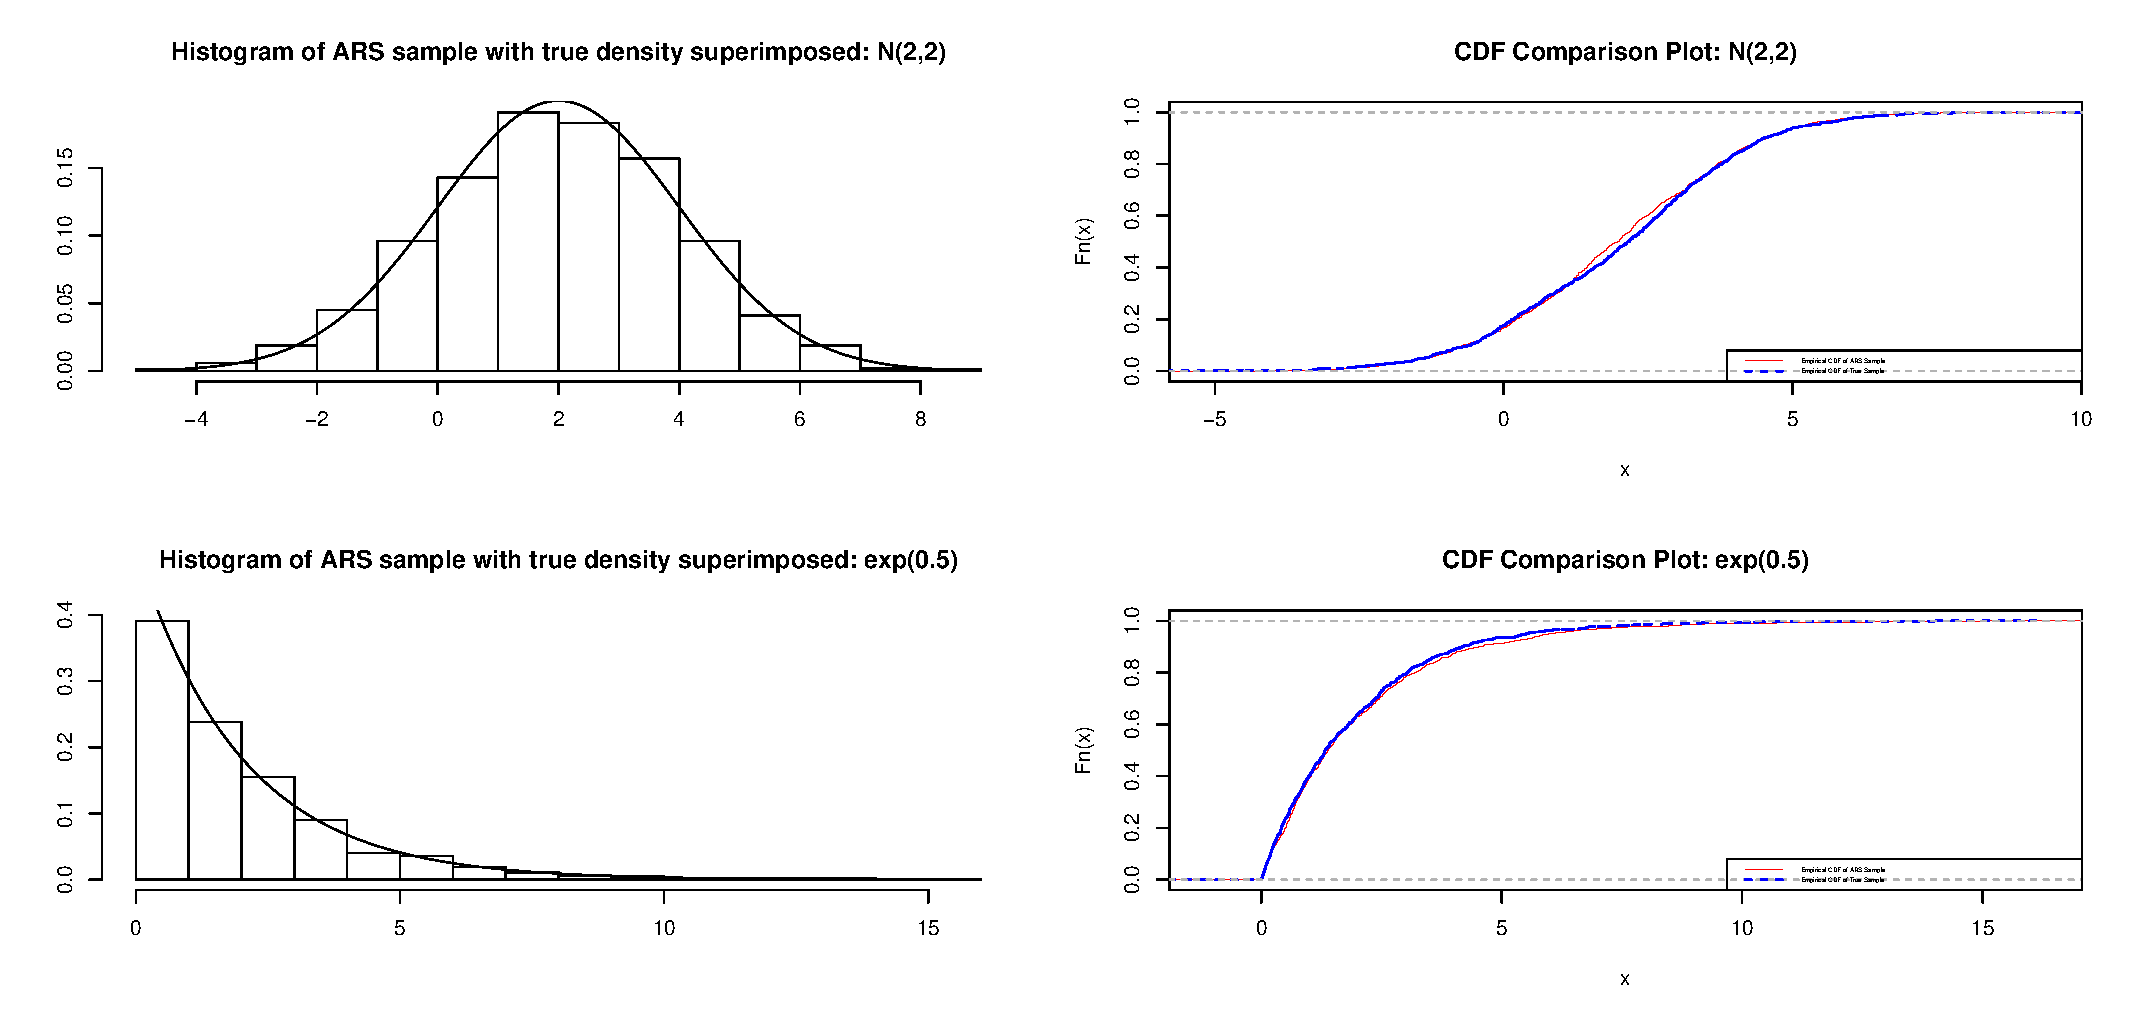
\includegraphics[scale=0.45]{plot1.pdf}\\

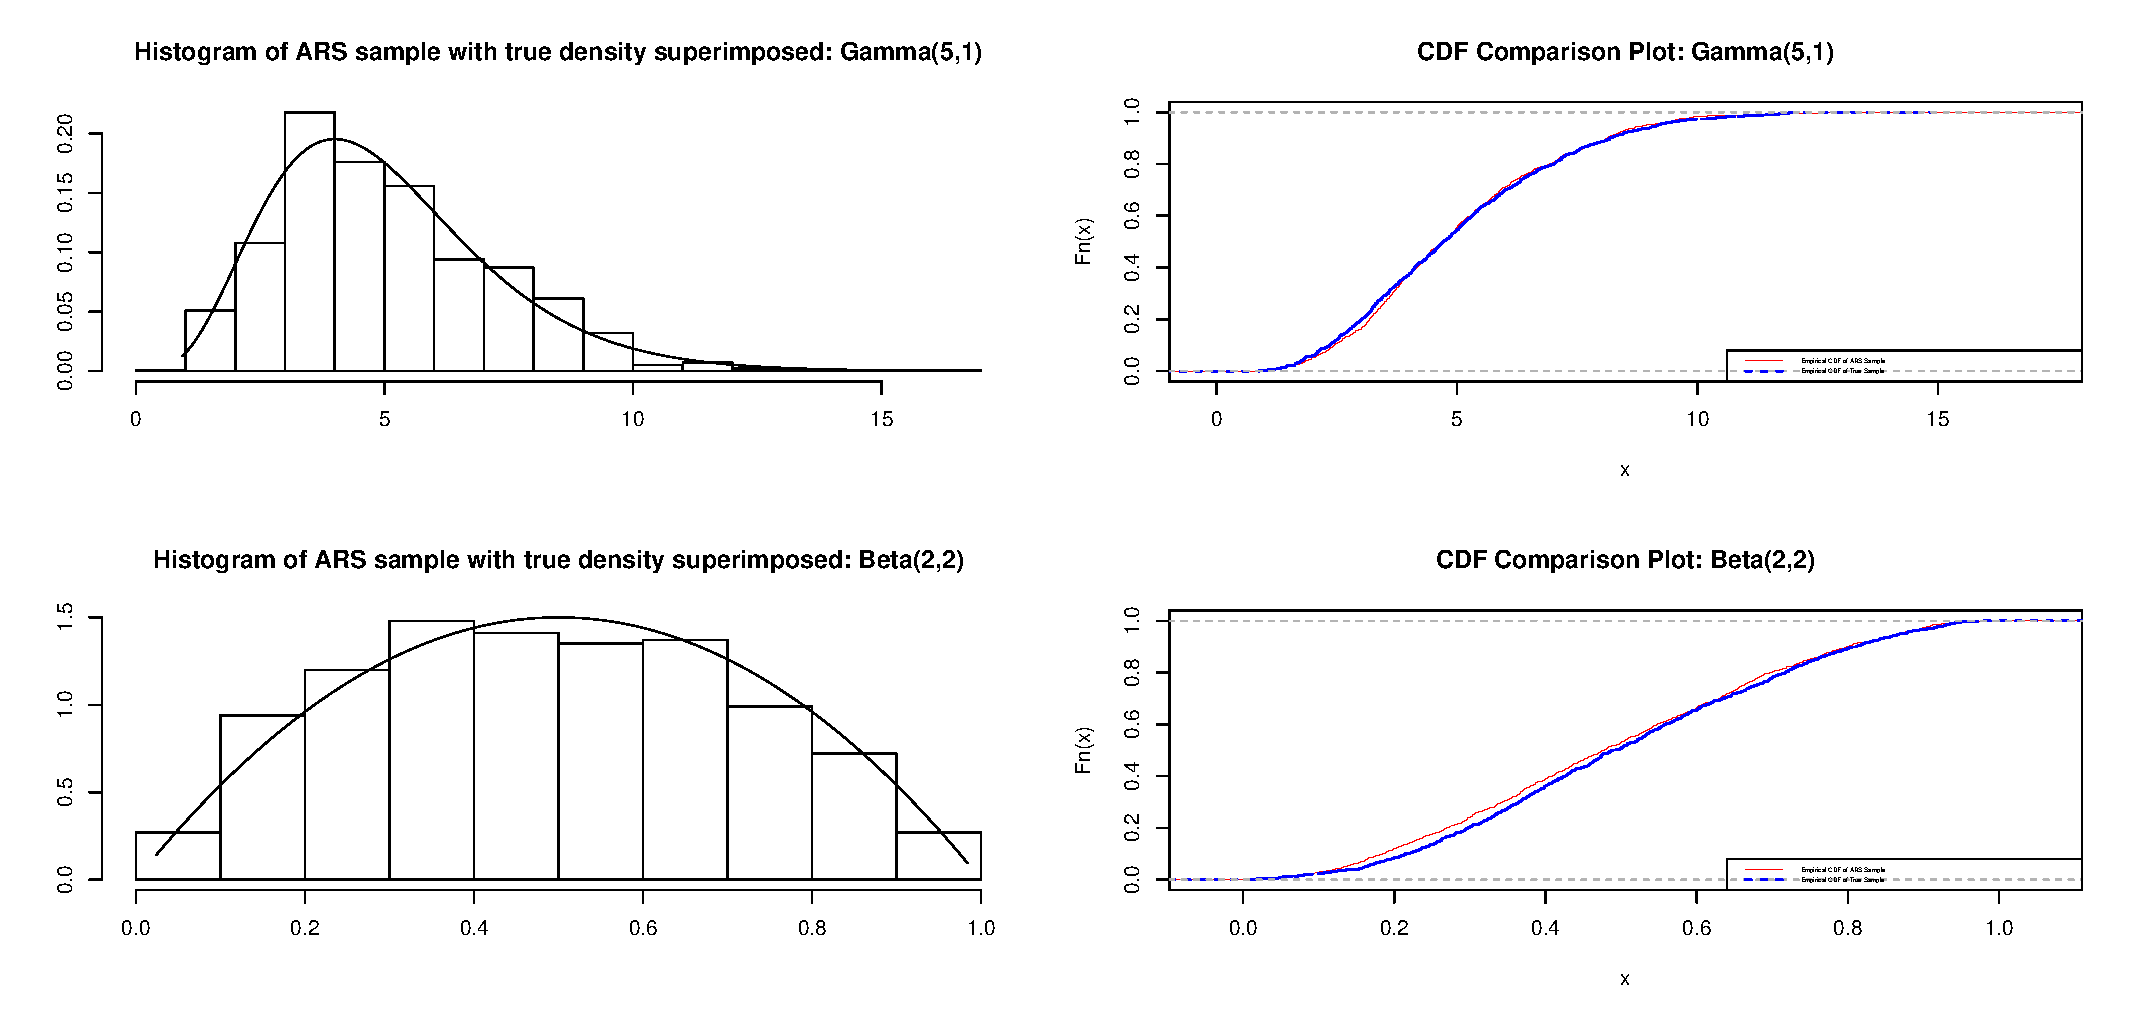
\includegraphics[scale=0.45]{plot4.pdf}


\section{Reflection and Group Dynamics}
We broke up the work in such a way that a single person started a step of the project, pushed his or her work to the GitHub repository, and solicited input, adjustments, and edits from the other team members.  In the above section (2), we mentioned individuals who started certain portions of the code; in addition, Matt took the lead as primary, initial author of this reflection paper and Ying did a bit of debugging work on the ARS code related to the domains of the densities.  However, it should be noted that everyone was involved in every piece of this project, and nothing can be uniquely attributed to a single group member.  Our team collaborated using GitHub, developing a unified naming convention for all files and folders in the repository. Our code also follows a standard naming convention practice.  We also communicated daily by email to update each other on our progress when the next stage of work was ready for the next person. The final pieces that we are turning in truly represent a full group effort. 

R Code submitted on bSpace by: M. Boyas

\end{document}